\section{Overview}
\label{sec:overview}

doomacracy is a computer built in one Cyclone II FPGA on a Terasic DE1 board. It has a pipelined RISC-V CPU, two caches, three memory controllers, a VGA output, a PS/2 keyboard input, a UART and a JTAG link to the host. All logic uses the 50 MHz board clock. The machine runs two programs: shareware Doom on bare metal, and a Linux kernel without an MMU.

This guide describes the hardware. Each section names the VHDL file that it describes. The files are in \src{rtl/}. The cycle counts come from the RTL or from the cycle model in the emulator (\src{emu/}).

\subsection{Block diagram}

Figure~\ref{fig:soc} shows the blocks. The CPU has an instruction port and a data port. Each port connects to an 8 KB cache. The two caches share one bus, \texttt{membus}. The bus sends each transaction to one of five slaves. Address bits 31:28 select the slave.

The video block does not use the bus. It reads the framebuffer through a second port on the SRAM controller.

\begin{figure}[H]
  \centering
  \begin{tikzpicture}[font=\small, x=1cm, y=1cm]
    \node[blk, minimum width=2.0cm, minimum height=2.6cm] (cpu) at (0,0) {CPU\\RV32IMA\\pipeline};
    \node[ram, minimum width=1.8cm] (ic) at (3.0,0.9)  {I-cache\\8 KB};
    \node[ram, minimum width=1.8cm] (dc) at (3.0,-0.9) {D-cache\\8 KB};
    \node[blk, minimum width=1.3cm, minimum height=6.6cm] (bus) at (5.7,0) {membus};
    \draw[sig] (1.0,0.9) -- (ic.west);
    \draw[bidir] (1.0,-0.9) -- (dc.west);
    \draw[bidir] (ic.east) -- (5.05,0.9);
    \draw[bidir] (dc.east) -- (5.05,-0.9);

    \foreach \s/\y/\t in {rom/2.6/{boot ROM, 4 KB}, sram/1.3/{SRAM controller}, sdram/0/{SDRAM controller},
                          flash/-1.3/{flash controller}, io/-2.6/{I/O registers}}
      \node[blk, minimum width=2.9cm, minimum height=0.8cm] (\s) at (9.3,\y) {\t};
    \foreach \s/\a in {rom/0x0, sram/0x1, sdram/{0x2, 0x8}, flash/0x3, io/0xF} {
      \draw[bidir] (\s.west -| bus.east) -- (\s.west);
      \node[above, lbl] at ($(\s.west -| bus.east)!0.5!(\s.west)$) {\texttt{\a}};
    }

    \node[blk, minimum width=1.4cm] (vid) at (12.3,1.3) {video};
    \draw[sig] (sram.east) -- (vid.west);
    \node[above, lbl, align=center] at (11.2,1.3) {private\\port};
    \draw[sig] (vid.south) -- ++(0,-0.9) node[below] {VGA};
  \end{tikzpicture}
  \caption{The system on chip. Each bus link shows the value of address bits 31:28 that selects the slave.}
  \label{fig:soc}
\end{figure}

\subsection{Full block diagram}
\label{sec:fullblock}

Figure~\ref{fig:full} shows the CPU and the system in one diagram. The diagram shows the data paths. It does not show these items:

\begin{itemize}
  \item The pipeline registers between the stages. Section~\ref{sec:pipeline} shows them.
  \item The control signals from the instruction decoder to the multiplexers and the units.
  \item The AMO unit in MEM and the store lane logic. Section~\ref{sec:alu} shows them.
\end{itemize}

The three horizontal buses in the CPU are the operand buses: rs1, rs2 and the immediate. A dot shows a connection to a bus. A line that crosses a bus without a dot is not connected to it.

\begin{landscape}
\begin{figure}[p]
  \centering
  \begin{tikzpicture}[x=1cm, y=1cm, font=\scriptsize,
      dot/.style={circle, fill, inner sep=1.3pt},
      rail/.style={double, double distance=1.8pt, line width=0.5pt}]

    % ================================================================ CPU
    \draw[dashed, line width=0.6pt] (0,0.35) rectangle (9.9,14.75);
    \node[align=center, font=\small] at (8.6,1.3) {CPU core\\\src{rtl/cpu.vhd}};

    % ---- fetch
    \node[mux, minimum height=1.4cm, minimum width=0.5cm] (pcmux) at (1.6,13.5) {};
    \node[below, font=\tiny] at (2.55,13.45) {PC MUX};
    \node[pblk, minimum width=1.8cm, minimum height=0.6cm] (pc) at (4.2,13.5) {Program counter};
    \draw[pbus] (1.85,13.5) -- (pc.west);
    \node[pblk, minimum width=0.7cm, minimum height=0.36cm] (p4) at (3.2,14.35) {$+4$};
    \draw[rail] (5.6,13.5) -- (5.6,14.35) -- (p4.east);
    \draw[pbus] (p4.west) -- (0.9,14.35) -- (0.9,13.95) -- (1.35,13.95);

    \node[pblk, minimum width=1.8cm, minimum height=0.7cm] (pd) at (8.6,12.3) {Predecode};
    \foreach \i in {0,...,3}
      \node[pblk, minimum width=1.4cm, minimum height=0.28cm, font=\tiny] (st\i) at (6.3,{12.07-0.28*\i}) {STACK \i};
    \draw[pbi] (7.0,12.08) -- (7.7,12.08);
    \draw[pbus] (7.7,12.45) -- (0.9,12.45) -- (0.9,13.05) -- (1.35,13.05);
    \node[above] at (3.6,12.45) {predicted target};

    \node[pblk, minimum width=1.8cm, minimum height=0.8cm] (iq) at (8.6,10.9) {Instruction\\queue (2)};
    \draw[pbus] (pd.south) -- (iq.north);
    \node[pblk, minimum width=2.6cm, minimum height=1.0cm] (dec) at (8.4,9.3) {Instruction\\decode \& control};
    \draw[pbus] (8.6,10.5) -- (8.6,9.8);

    % ---- register file and forwarding
    \node[pblk, minimum width=2.4cm, minimum height=1.3cm] (rf) at (2.3,9.3) {Register file\\32 $\times$ 32 bits\\(M4K RAM)};
    \draw[pbus] (dec.west) -- (rf.east);
    \node[above] at (5.3,9.3) {rs1, rs2, rd};
    \bw[below]{5.3,9.3}{3 $\times$ 5}
    \draw[line width=0.6pt, fill=white] (1.0,7.95) -- (3.6,7.95) -- (3.3,7.45) -- (1.3,7.45) -- cycle;
    \node at (2.3,7.7) {Forward MUX};
    \draw[pbus] (1.8,8.65) -- (1.8,7.95);
    \draw[pbus] (2.8,8.65) -- (2.8,7.95);

    % ---- operand buses (drawn first, so later lines cross over them)
    \draw[rail] (1.15,6.7) -- (7.8,6.7);
    \draw[rail] (2.3,6.4) -- (9.0,6.4);
    \draw[rail] (3.0,6.1) -- (8.4,6.1);
    \node[right] at (7.85,6.78) {rs1};
    \node[right] at (5.1,5.82) {imm};
    \draw[rail] (1.8,7.45) -- (1.8,6.7);   \node[dot] at (1.8,6.7) {};
    \draw[rail] (2.8,7.45) -- (2.8,6.4);   \node[dot] at (2.8,6.4) {};
    \draw[rail] (8.4,8.8) -- (8.4,6.1);    \node[dot] at (8.4,6.1) {};

    % ---- execute units
    \draw[line width=0.6pt, fill=white] (1.9,5.62) -- (3.4,5.62) -- (3.1,5.18) -- (2.2,5.18) -- cycle;
    \node[font=\tiny] at (2.65,5.4) {MUX};
    \draw[pbus] (2.3,6.4) -- (2.3,5.62);   \node[dot] at (2.3,6.4) {};
    \draw[pbus] (3.0,6.1) -- (3.0,5.62);   \node[dot] at (3.0,6.1) {};
    \draw[line width=0.6pt, fill=white] (0.7,4.6) -- (1.6,4.6) -- (1.9,4.35) -- (2.2,4.6) -- (3.1,4.6) -- (2.6,3.8) -- (1.2,3.8) -- cycle;
    \node at (1.9,4.05) {ALU};
    \draw[pbus] (1.15,6.7) -- (1.15,4.6);  \node[dot] at (1.15,6.7) {};
    \draw[pbus] (2.65,5.18) -- (2.65,4.6);

    \node[pblk, minimum width=1.5cm, minimum height=0.9cm] (md) at (4.4,4.4) {Multiply\\divide};
    \draw[pbus] (4.1,6.7) -- (4.1,4.85);   \node[dot] at (4.1,6.7) {};
    \draw[pbus] (4.7,6.4) -- (4.7,4.85);   \node[dot] at (4.7,6.4) {};
    \node[pblk, minimum width=1.4cm, minimum height=0.9cm] (br) at (6.2,4.4) {Branch\\compare};
    \draw[pbus] (5.9,6.7) -- (5.9,4.85);   \node[dot] at (5.9,6.7) {};
    \draw[pbus] (6.5,6.4) -- (6.5,4.85);   \node[dot] at (6.5,6.4) {};
    \node[pblk, minimum width=1.5cm, minimum height=0.9cm] (ad) at (8.1,4.4) {Address\\adder};
    \draw[pbus] (7.8,6.7) -- (7.8,4.85);   \node[dot] at (7.8,6.7) {};
    \draw[pbus] (8.4,6.1) -- (8.4,4.85);

    % ---- CSRs, traps, result
    \node[pblk, minimum width=2.2cm, minimum height=1.0cm] (csr) at (6.3,2.6) {CSRs, traps,\\next PC};
    \draw[pwire] (6.2,3.95) -- (6.2,3.1);
    \node[pblk, minimum width=1.5cm, minimum height=0.5cm] (la) at (8.3,3.5) {Load align};
    \draw[line width=0.6pt, fill=white] (1.4,2.85) -- (4.8,2.85) -- (4.5,2.35) -- (1.7,2.35) -- cycle;
    \node at (3.0,2.6) {Result MUX};
    \draw[pbus] (1.9,3.8) -- (1.9,2.85);
    \draw[pbus] (3.9,3.95) -- (3.9,2.85);
    \draw[pbus] (la.west) -- (4.45,3.5) -- (4.45,2.85);
    \draw[pbus] (csr.west) -- (4.65,2.6);
    % result bus: back to the register file and the forward MUX
    \draw[pbus] (3.1,2.35) -- (3.1,1.25) -- (0.65,1.25) -- (0.65,9.3) -- (rf.west);
    \draw[pbus] (0.65,7.7) -- (1.15,7.7);  \node[dot] at (0.65,7.7) {};
    \node[above] at (1.9,1.25) {result bus};
    \bw[below]{2.4,1.25}{32}
    % redirect: to the PC MUX
    \draw[pbus] (6.3,2.1) -- (6.3,0.75) -- (0.3,0.75) -- (0.3,13.5) -- (1.35,13.5);
    \node[above] at (4.9,0.75) {redirect target};
    \bw[below]{4.2,0.75}{32}

    % ================================================================ caches and bus
    \node[pblk, minimum width=1.8cm, minimum height=2.0cm] (ic) at (12.2,12.9) {I-cache\\8 KB\\512 lines};
    \node[pblk, minimum width=1.8cm, minimum height=3.4cm] (dc) at (12.2,4.9) {D-cache\\8 KB\\512 lines\\[4pt]write buffer\\4 entries};
    \draw[pbus] (pc.east) -- (11.3,13.5);
    \node[above] at (7.6,13.5) {fetch address};
    \bw[above]{10.65,13.5}{32}
    \draw[pbus] (11.3,12.3) -- (pd.east);
    \node[below, fill=white, inner sep=1.5pt] at (10.62,12.12) {instruction};
    \bw[above]{10.65,12.3}{32}
    \draw[pbus] (9.0,6.4) -- (11.3,6.4);
    \node[below] at (10.6,6.3) {store data};
    \node[above] at (9.35,6.42) {rs2};
    \bw[above]{10.65,6.4}{32}
    \draw[pbus] (ad.east) -- (11.3,4.4);
    \node[below] at (10.6,4.3) {address};
    \bw[above]{10.65,4.4}{32}
    \draw[pbus] (11.3,3.5) -- (la.east);
    \node[below] at (10.6,3.4) {load data};
    \bw[above]{10.65,3.5}{32}

    \node[pblk, minimum width=1.0cm, minimum height=10.1cm] (bus) at (14.3,8.95) {\rotatebox{90}{membus (one transaction at a time)}};
    \draw[pbi] (ic.east) -- (13.8,12.9);
    \draw[pbi] (dc.east) -- (13.8,4.9);

    % ================================================================ slaves
    \node[pblk, minimum width=2.2cm, minimum height=0.8cm] (rom)   at (16.7,13.4) {Boot ROM\\4 KB};
    \node[pblk, minimum width=2.2cm, minimum height=1.1cm] (sram)  at (16.7,11.5) {SRAM\\controller};
    \node[pblk, minimum width=2.2cm, minimum height=1.1cm] (sdram) at (16.7,8.6)  {SDRAM\\controller};
    \node[pblk, minimum width=2.2cm, minimum height=1.1cm] (flash) at (16.7,6.6)  {Flash\\controller};
    \node[pblk, minimum width=2.2cm, minimum height=4.8cm] (io)    at (16.7,3.2)  {I/O registers\\[3pt]timers\\CLINT, PLIC\\16550\\syscon\\keyboard FIFO};
    \foreach \y/\a in {13.4/0x0, 11.5/0x1, 8.6/0x2, 6.6/0x3, 4.6/0xF} {
      \draw[pbi] (14.8,\y) -- (15.6,\y);
      \node[above, font=\tiny\ttfamily, inner sep=2.5pt] at (15.2,\y) {\a};
    }
    \node[below, font=\tiny\ttfamily, inner sep=2.5pt] at (15.2,8.6) {0x8};

    % ================================================================ device blocks and pins
    \node[pblk, minimum width=1.6cm, minimum height=0.9cm] (vid)  at (19.1,10.0) {Video};
    \node[pblk, minimum width=1.6cm, minimum height=0.7cm] (uart) at (19.1,5.0)  {UART};
    \node[pblk, minimum width=1.6cm, minimum height=0.7cm] (ps2)  at (19.1,3.9)  {PS/2 receiver};
    \node[pblk, minimum width=1.6cm, minimum height=0.8cm] (jtag) at (19.1,2.8)  {JTAG loader\\and console};
    \draw[pbi] (17.4,10.95) -- (17.4,10.0) -- (vid.west);
    \node[below, font=\tiny] at (17.75,9.95) {video port};
    \draw[pbi] (17.8,5.0) -- (uart.west);
    \draw[pbus] (ps2.west) -- (17.8,3.9);
    \draw[pbi] (17.8,2.8) -- (jtag.west);

    % pins: \y, label, kind (o = output, i = input, b = both), source x
    \foreach \y/\t/\k/\x in {
        11.9/{SRAM\_ADDR[17:0]}/o/17.8, 11.5/{SRAM\_DQ[15:0]}/b/17.8, 11.1/{SRAM control}/o/17.8,
        10.2/{VGA\_R, G, B [3:0]}/o/19.9, 9.8/{VGA\_HS, VGA\_VS}/o/19.9,
        9.0/{DRAM\_ADDR, BA}/o/17.8, 8.6/{DRAM\_DQ[15:0]}/b/17.8, 8.2/{DRAM control, CLK}/o/17.8,
        7.0/{FL\_ADDR[21:0]}/o/17.8, 6.6/{FL\_DQ[7:0]}/b/17.8, 6.2/{FL control}/o/17.8,
        5.2/{UART\_TXD}/o/19.9, 4.8/{UART\_RXD}/i/19.9,
        4.1/{PS2\_CLK}/i/19.9, 3.7/{PS2\_DAT}/i/19.9,
        2.8/{USB-Blaster}/b/19.9,
        1.9/{LEDR, LEDG}/o/17.8, 1.5/{HEX3 to HEX0}/o/17.8, 1.1/{SW[9:0], KEY[3:1]}/i/17.8} {
      \node[pin] (p) at (20.6,\y) {};
      \node[right, font=\tiny\ttfamily, inner sep=2pt] at (20.72,\y) {\t};
      \if\k o\draw[pwire] (\x,\y) -- (p.west);\fi
      \if\k i\draw[pwire] (p.west) -- (\x,\y);\fi
      \if\k b\draw[line width=0.5pt, {Latex[length=1.6mm]}-{Latex[length=1.6mm]}] (\x,\y) -- (p.west);\fi
    }

    % ================================================================ reset, clock, interrupts
    \node[pblk, minimum width=2.4cm, minimum height=0.9cm] (rst) at (12.6,1.3) {Reset and clock\\50 MHz};
    \node[pin] (pck) at (11.7,0.3) {};
    \node[right, font=\tiny\ttfamily, inner sep=2pt] at (11.82,0.3) {CLOCK\_50};
    \node[pin] (pk0) at (13.5,0.3) {};
    \node[right, font=\tiny\ttfamily, inner sep=2pt] at (13.62,0.3) {KEY[0]};
    \draw[pwire] (pck.north) -- (11.7,0.85);
    \draw[pwire] (pk0.north) -- (13.5,0.85);
    \draw[pwire] (rst.west) -- (9.9,1.3);
    \node[above, font=\tiny] at (10.65,1.3) {reset, clk};
    \draw[pwire] (15.6,2.4) -- (csr.east |- 0,2.4);
    \node[above, font=\tiny] at (12.8,2.4) {interrupts: MTIP, MSIP, MEIP};
    \draw[pwire] (15.6,1.3) -- (rst.east);
    \node[above, font=\tiny] at (14.7,1.3) {reboot};

    % ================================================================ legend
    \draw[pbus] (18.5,14.4) -- (19.3,14.4);
    \node[right] at (19.4,14.4) {bus, width in bits};
    \draw[pwire] (18.5,13.95) -- (19.3,13.95);
    \node[right] at (19.4,13.95) {single signals};
    \node[pin] at (18.9,13.5) {};
    \node[right] at (19.4,13.5) {FPGA pin};
    \node[dot] at (18.9,13.05) {};
    \node[right] at (19.4,13.05) {connection to a bus};
  \end{tikzpicture}
  \caption{The full block diagram}
  \label{fig:full}
\end{figure}
\end{landscape}


\subsection{Memory map}

Figure~\ref{fig:memmap} shows the address space. The first hex digit of an address selects the device. Thus the bus decoder compares only four bits.

The SDRAM is at two addresses. The firmware uses \texttt{0x2000\_0000}. Linux uses \texttt{0x8000\_0000}, because a RISC-V Linux kernel expects RAM at that address. The D-cache stores one tag for the two addresses of a word. A write through one address is visible through the other address.

\begin{figure}[H]
  \centering
  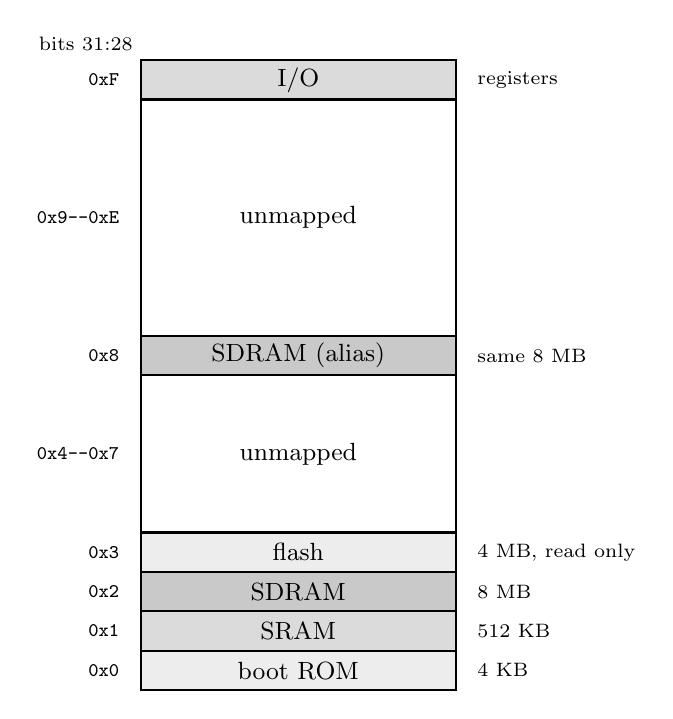
\begin{tikzpicture}[x=1cm, y=0.5cm, font=\small]
    \foreach \y/\h/\name/\base/\size/\shade in {
        0/1/boot ROM/0x0/4 KB/7,
        1/1/SRAM/0x1/512 KB/14,
        2/1/SDRAM/0x2/8 MB/21,
        3/1/flash/0x3/{4 MB, read only}/7,
        4/4/unmapped/0x4--0x7//0,
        8/1/SDRAM (alias)/0x8/same 8 MB/21,
        9/6/unmapped/0x9--0xE//0,
        15/1/{I/O}/0xF/registers/14} {
      \draw[thick, fill=black!\shade] (0,\y) rectangle (4.0,\y+\h);
      \node at (2.0,\y+\h/2) {\name};
      \node[left, font=\ttfamily\scriptsize] at (-0.15,\y+\h/2) {\base};
      \node[right, font=\scriptsize] at (4.15,\y+\h/2) {\size};
    }
    \node[above] at (-0.7,16) {\scriptsize bits 31:28};
  \end{tikzpicture}
  \hspace{1.0cm}
  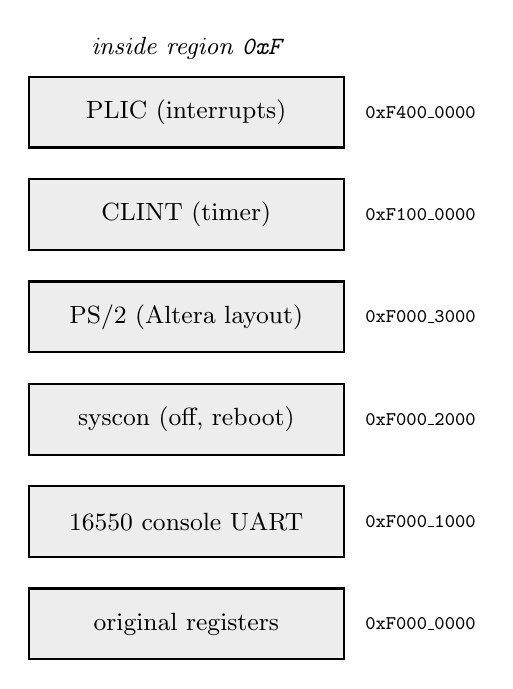
\begin{tikzpicture}[x=1cm, y=0.5cm, font=\small]
    \foreach \y/\name/\base in {
        0/original registers/0xF000\_0000,
        2.6/16550 console UART/0xF000\_1000,
        5.2/{syscon (off, reboot)}/0xF000\_2000,
        7.8/{PS/2 (Altera layout)}/0xF000\_3000,
        10.4/CLINT (timer)/0xF100\_0000,
        13.0/PLIC (interrupts)/0xF400\_0000} {
      \draw[thick, fill=black!7] (0,\y) rectangle (4.0,\y+1.8);
      \node at (2.0,\y+0.9) {\name};
      \node[right, font=\ttfamily\scriptsize] at (4.15,\y+0.9) {\base};
    }
    \node[above, font=\small\itshape] at (2.0,15.0) {inside region \texttt{0xF}};
  \end{tikzpicture}
  \caption{The memory map. Left: the regions that address bits 31:28 select, with low addresses at the bottom. Right: the devices in the I/O region.}
  \label{fig:memmap}
\end{figure}

Table~\ref{tab:memmap} gives the size and the use of each region.

\begin{guidetable}{Memory regions}{memmap}{l l l l l}
base & size & device & D-cache & notes \\
\midrule
\texttt{0x0000\_0000} & 4 KB & boot ROM (M4K) & uncached & reset vector at 0 \\
\texttt{0x1000\_0000} & 512 KB & 16-bit async SRAM & cached & framebuffers, hot code \\
\texttt{0x2000\_0000} & 8 MB & SDRAM & cached & cold code, heap \\
\texttt{0x3000\_0000} & 4 MB & 8-bit NOR flash & uncached & firmware and WAD \\
\texttt{0x8000\_0000} & 8 MB & SDRAM alias & cached & RAM for Linux \\
\texttt{0xF000\_0000} & -- & I/O & uncached & word access only \\
\end{guidetable}

The ``D-cache'' column applies to loads and stores. The I-cache caches all instruction fetches.

\subsection{FPGA resources}

The EP2C20 has 18,752 logic elements, 52 M4K RAM blocks (4 Kbit each) and 26 multipliers (18 $\times$ 18). All RAMs in the design are M4K blocks: the two caches, the register file, the boot ROM, the video line buffer and the palette.

An M4K block has a register on its read address. The data comes out one cycle after the address goes in. This property sets the structure of the pipeline (Section~\ref{sec:pipeline}).

\subsection{Sections}

\begin{itemize}
  \item Sections~\ref{sec:isa} to~\ref{sec:traps}: the CPU. Instruction set, pipeline, ALU, multiply and divide, traps.
  \item Section~\ref{sec:memory}: the caches, the bus and the memory controllers.
  \item Section~\ref{sec:videoio}: video and the I/O devices.
  \item Section~\ref{sec:boot}: reset, the boot ROM and the software.
\end{itemize}
